\documentclass[tikz,border=1pt]{standalone}
\usepackage[T1]{fontenc}
\usepackage{amsmath}
\usepackage{newtxtext,newtxmath}
\usepackage{pifont}
\usetikzlibrary{arrows.meta,positioning,calc,fit,backgrounds,patterns,patterns.meta,shapes.geometric,shapes.misc}

% Okabe-Ito colourblind-safe palette (one colour per method in every figure)
\definecolor{oiBlue}{HTML}{0072B2}
\definecolor{oiVermilion}{HTML}{D55E00}
\definecolor{oiGreen}{HTML}{009E73}
\definecolor{oiOrange}{HTML}{E69F00}
\definecolor{oiPurple}{HTML}{CC79A7}
\definecolor{oiSky}{HTML}{56B4E9}
\definecolor{oiYellow}{HTML}{F0E442}
\definecolor{oiGrey}{HTML}{8C8C8C}
\definecolor{oiGrid}{HTML}{D9D9D9}
\definecolor{oiInk}{HTML}{1A1A1A}

\newcommand{\okmark}{\textcolor{oiGreen!70!black}{\ding{51}}}
\newcommand{\badmark}{\textcolor{oiVermilion}{\ding{55}}}
\newcommand{\cellfont}{\fontsize{6.5}{7.6}\selectfont}

\tikzset{
  >={Latex[length=1.7mm,width=1.4mm]},
  flow/.style={->, line width=0.6pt, draw=oiInk},
  hatch/.style={pattern={Lines[angle=45,distance=2.4pt,line width=0.35pt]}, pattern color=black!28},
}

\tikzset{subcap/.style={font=\footnotesize, anchor=north, inner sep=0pt}}
\begin{document}
\renewcommand{\cellfont}{\fontsize{8.5}{9.6}\selectfont}
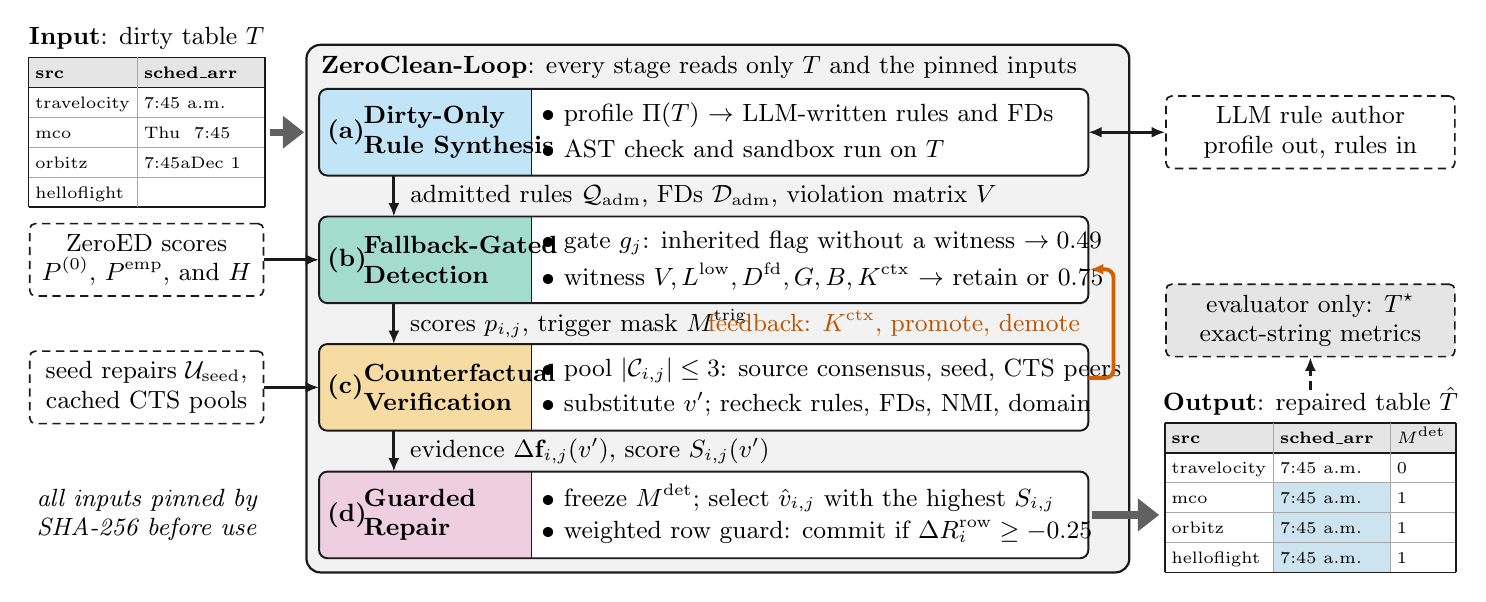
\begin{tikzpicture}[x=1cm,y=1cm, font=\fontsize{9}{10.6}\selectfont,
  pin/.style={draw=oiInk, line width=0.6pt, densely dashed, rounded corners=2pt, fill=white, align=center, inner sep=2pt, minimum height=0.92cm},
  block/.style={line width=2.6pt, draw=black!62, -{Triangle[length=2.7mm,width=4.0mm]}},
  art/.style={->, line width=1.0pt, draw=oiInk}]
\draw[rounded corners=5pt, line width=0.8pt, draw=oiInk, fill=black!5] (3.53,0) rectangle (13.98,6.700);
\node[anchor=west, inner sep=0pt] at (3.710,6.410) {\textbf{ZeroClean-Loop}: every stage reads only $T$ and the pinned inputs};
\begin{scope}
\clip[rounded corners=3pt] (3.690,5.040) rectangle (13.460,6.140);
\fill[white] (3.690,5.040) rectangle (13.460,6.140);
\fill[oiSky!36] (3.690,5.040) rectangle (6.390,6.140);
\end{scope}
\draw[rounded corners=3pt, line width=0.7pt, draw=oiInk] (3.690,5.040) rectangle (13.460,6.140);
\draw[line width=0.5pt, draw=oiInk] (6.390,5.040) -- (6.390,6.140);
\node[anchor=west, inner sep=0pt, font=\fontsize{9}{10.6}\selectfont\bfseries] at (3.790,5.590) {(a)};
\node[anchor=west, inner sep=0pt, align=left, font=\fontsize{9}{10.6}\selectfont\bfseries] at (4.250,5.590) {Dirty-Only\\Rule Synthesis};
\node[anchor=west, inner sep=0pt] at (6.520,5.805) {\textbullet~profile $\Pi(T)$ $\rightarrow$ LLM-written rules and FDs};
\node[anchor=west, inner sep=0pt] at (6.520,5.375) {\textbullet~AST check and sandbox run on $T$};
\coordinate (aW) at (3.690,5.590); \coordinate (aE) at (13.460,5.590);
\begin{scope}
\clip[rounded corners=3pt] (3.690,3.420) rectangle (13.460,4.520);
\fill[white] (3.690,3.420) rectangle (13.460,4.520);
\fill[oiGreen!36] (3.690,3.420) rectangle (6.390,4.520);
\end{scope}
\draw[rounded corners=3pt, line width=0.7pt, draw=oiInk] (3.690,3.420) rectangle (13.460,4.520);
\draw[line width=0.5pt, draw=oiInk] (6.390,3.420) -- (6.390,4.520);
\node[anchor=west, inner sep=0pt, font=\fontsize{9}{10.6}\selectfont\bfseries] at (3.790,3.970) {(b)};
\node[anchor=west, inner sep=0pt, align=left, font=\fontsize{9}{10.6}\selectfont\bfseries] at (4.250,3.970) {Fallback-Gated\\Detection};
\node[anchor=west, inner sep=0pt] at (6.520,4.185) {\textbullet~gate $g_j$: inherited flag without a witness $\rightarrow 0.49$};
\node[anchor=west, inner sep=0pt] at (6.520,3.755) {\textbullet~witness $V, L^{\mathrm{low}}, D^{\mathrm{fd}}, G, B, K^{\mathrm{ctx}}$ $\rightarrow$ retain or $0.75$};
\coordinate (bW) at (3.690,3.970); \coordinate (bE) at (13.460,3.970);
\begin{scope}
\clip[rounded corners=3pt] (3.690,1.800) rectangle (13.460,2.900);
\fill[white] (3.690,1.800) rectangle (13.460,2.900);
\fill[oiOrange!36] (3.690,1.800) rectangle (6.390,2.900);
\end{scope}
\draw[rounded corners=3pt, line width=0.7pt, draw=oiInk] (3.690,1.800) rectangle (13.460,2.900);
\draw[line width=0.5pt, draw=oiInk] (6.390,1.800) -- (6.390,2.900);
\node[anchor=west, inner sep=0pt, font=\fontsize{9}{10.6}\selectfont\bfseries] at (3.790,2.350) {(c)};
\node[anchor=west, inner sep=0pt, align=left, font=\fontsize{9}{10.6}\selectfont\bfseries] at (4.250,2.350) {Counterfactual\\Verification};
\node[anchor=west, inner sep=0pt] at (6.520,2.565) {\textbullet~pool $|\mathcal{C}_{i,j}| \le 3$: source consensus, seed, CTS peers};
\node[anchor=west, inner sep=0pt] at (6.520,2.135) {\textbullet~substitute $v'$; recheck rules, FDs, NMI, domain};
\coordinate (cW) at (3.690,2.350); \coordinate (cE) at (13.460,2.350);
\begin{scope}
\clip[rounded corners=3pt] (3.690,0.180) rectangle (13.460,1.280);
\fill[white] (3.690,0.180) rectangle (13.460,1.280);
\fill[oiPurple!36] (3.690,0.180) rectangle (6.390,1.280);
\end{scope}
\draw[rounded corners=3pt, line width=0.7pt, draw=oiInk] (3.690,0.180) rectangle (13.460,1.280);
\draw[line width=0.5pt, draw=oiInk] (6.390,0.180) -- (6.390,1.280);
\node[anchor=west, inner sep=0pt, font=\fontsize{9}{10.6}\selectfont\bfseries] at (3.790,0.730) {(d)};
\node[anchor=west, inner sep=0pt, align=left, font=\fontsize{9}{10.6}\selectfont\bfseries] at (4.250,0.730) {Guarded\\Repair};
\node[anchor=west, inner sep=0pt] at (6.520,0.945) {\textbullet~freeze $M^{\mathrm{det}}$; select $\hat{v}_{i,j}$ with the highest $S_{i,j}$};
\node[anchor=west, inner sep=0pt] at (6.520,0.515) {\textbullet~weighted row guard: commit if $\Delta R_i^{\mathrm{row}} \ge -0.25$};
\coordinate (dW) at (3.690,0.730); \coordinate (dE) at (13.460,0.730);
\draw[art] (4.640,5.040) -- (4.640,4.520);
\node[anchor=west, inner sep=0pt] at (4.840,4.780) {admitted rules $\mathcal{Q}_{\mathrm{adm}}$, FDs $\mathcal{D}_{\mathrm{adm}}$, violation matrix $V$};
\draw[art] (4.640,3.420) -- (4.640,2.900);
\node[anchor=west, inner sep=0pt] at (4.840,3.160) {scores $p_{i,j}$, trigger mask $M^{\mathrm{trig}}$};
\draw[art] (4.640,1.800) -- (4.640,1.280);
\node[anchor=west, inner sep=0pt] at (4.840,1.540) {evidence $\Delta\mathbf{f}_{i,j}(v')$, score $S_{i,j}(v')$};
\draw[->, line width=1.4pt, draw=oiVermilion, rounded corners=3pt] (13.460,2.470) -- (13.780,2.470) -- (13.780,3.850) -- (13.480,3.850);
\node[anchor=east, inner sep=0pt, text=oiVermilion!88!black] at (13.360,3.160) {feedback: $K^{\mathrm{ctx}}$, promote, demote};
\fill[white] (0.000,4.640) rectangle (3.000,6.540);
\fill[black!10] (0.000,6.160) rectangle (3.000,6.540);
\node[anchor=base west, inner sep=0pt] at (0.080,6.275) {\cellfont\bfseries src};
\node[anchor=base west, inner sep=0pt] at (1.460,6.275) {\cellfont\bfseries sched\_arr};
\node[anchor=base west, inner sep=0pt] at (0.080,5.895) {\cellfont travelocity};
\node[anchor=base west, inner sep=0pt] at (1.460,5.895) {\cellfont 7:45 a.m.};
\node[anchor=base west, inner sep=0pt] at (0.080,5.515) {\cellfont mco};
\node[anchor=base west, inner sep=0pt] at (1.460,5.515) {\cellfont Thu ~7:45};
\node[anchor=base west, inner sep=0pt] at (0.080,5.135) {\cellfont orbitz};
\node[anchor=base west, inner sep=0pt] at (1.460,5.135) {\cellfont 7:45aDec 1};
\node[anchor=base west, inner sep=0pt] at (0.080,4.755) {\cellfont helloflight};
\node[anchor=base west, inner sep=0pt] at (1.460,4.755) {\cellfont $\varnothing$};
\draw[line width=0.6pt, draw=oiInk] (0.000,6.540) -- (3.000,6.540);
\draw[line width=0.6pt, draw=oiInk] (0.000,6.160) -- (3.000,6.160);
\draw[line width=0.25pt, draw=black!35] (0.000,5.780) -- (3.000,5.780);
\draw[line width=0.25pt, draw=black!35] (0.000,5.400) -- (3.000,5.400);
\draw[line width=0.25pt, draw=black!35] (0.000,5.020) -- (3.000,5.020);
\draw[line width=0.6pt, draw=oiInk] (0.000,4.640) -- (3.000,4.640);
\draw[line width=0.25pt, draw=black!35] (1.380,6.540) -- (1.380,4.640);
\draw[line width=0.6pt, draw=oiInk] (0.000,6.540) -- (0.000,4.640) (3.000,6.540) -- (3.000,4.640);
\node[anchor=south, inner sep=0pt] at (1.500,6.630) {\textbf{Input}: dirty table $T$};
\draw[block] (3.070,5.590) -- (3.500,5.590);
\node[pin, minimum width=2.97cm] (pinb) at (1.500,3.970) {ZeroED scores\\$P^{(0)}$, $P^{\mathrm{emp}}$, and $H$};
\draw[art] (pinb.east) -- (bW);
\node[pin, minimum width=2.97cm] (pinc) at (1.500,2.350) {seed repairs $\mathcal{U}_{\mathrm{seed}}$,\\cached CTS pools};
\draw[art] (pinc.east) -- (cW);
\node[inner sep=0pt, align=center, font=\fontsize{9}{10.6}\selectfont\itshape] at (1.500,0.730) {all inputs pinned by\\SHA-256 before use};
\node[pin, minimum width=3.67cm] (llm) at (16.280,5.590) {LLM rule author\\profile out, rules in};
\draw[art, <->] (aE) -- (llm.west);
\fill[white] (14.430,0.000) rectangle (18.130,1.900);
\fill[black!10] (14.430,1.520) rectangle (18.130,1.900);
\fill[oiBlue!20] (15.810,0.760) rectangle (17.290,1.140);
\fill[oiBlue!20] (15.810,0.380) rectangle (17.290,0.760);
\fill[oiBlue!20] (15.810,0.000) rectangle (17.290,0.380);
\node[anchor=base west, inner sep=0pt] at (14.510,1.635) {\cellfont\bfseries src};
\node[anchor=base west, inner sep=0pt] at (15.890,1.635) {\cellfont\bfseries sched\_arr};
\node[anchor=base west, inner sep=0pt] at (17.370,1.635) {\cellfont\bfseries $M^{\mathrm{det}}$};
\node[anchor=base west, inner sep=0pt] at (14.510,1.255) {\cellfont travelocity};
\node[anchor=base west, inner sep=0pt] at (15.890,1.255) {\cellfont 7:45 a.m.};
\node[anchor=base west, inner sep=0pt] at (17.370,1.255) {\cellfont 0};
\node[anchor=base west, inner sep=0pt] at (14.510,0.875) {\cellfont mco};
\node[anchor=base west, inner sep=0pt] at (15.890,0.875) {\cellfont 7:45 a.m.};
\node[anchor=base west, inner sep=0pt] at (17.370,0.875) {\cellfont 1};
\node[anchor=base west, inner sep=0pt] at (14.510,0.495) {\cellfont orbitz};
\node[anchor=base west, inner sep=0pt] at (15.890,0.495) {\cellfont 7:45 a.m.};
\node[anchor=base west, inner sep=0pt] at (17.370,0.495) {\cellfont 1};
\node[anchor=base west, inner sep=0pt] at (14.510,0.115) {\cellfont helloflight};
\node[anchor=base west, inner sep=0pt] at (15.890,0.115) {\cellfont 7:45 a.m.};
\node[anchor=base west, inner sep=0pt] at (17.370,0.115) {\cellfont 1};
\draw[line width=0.6pt, draw=oiInk] (14.430,1.900) -- (18.130,1.900);
\draw[line width=0.6pt, draw=oiInk] (14.430,1.520) -- (18.130,1.520);
\draw[line width=0.25pt, draw=black!35] (14.430,1.140) -- (18.130,1.140);
\draw[line width=0.25pt, draw=black!35] (14.430,0.760) -- (18.130,0.760);
\draw[line width=0.25pt, draw=black!35] (14.430,0.380) -- (18.130,0.380);
\draw[line width=0.6pt, draw=oiInk] (14.430,0.000) -- (18.130,0.000);
\draw[line width=0.25pt, draw=black!35] (15.810,1.900) -- (15.810,0.000);
\draw[line width=0.25pt, draw=black!35] (17.290,1.900) -- (17.290,0.000);
\draw[line width=0.6pt, draw=oiInk] (14.430,1.900) -- (14.430,0.000) (18.130,1.900) -- (18.130,0.000);
\node[anchor=south, inner sep=0pt] (olab) at (16.280,1.990) {\textbf{Output}: repaired table $\hat{T}$};
\draw[block] (13.510,0.730) -- (14.360,0.730);
\node[pin, fill=black!10, minimum width=3.67cm] (eval) at (16.280,3.200) {evaluator only: $T^{\star}$\\exact-string metrics};
\draw[->, line width=0.8pt, densely dashed, draw=oiInk] (16.280,2.320) -- (eval.south);
\end{tikzpicture}
\end{document}
